\documentclass[11pt,t]{beamer}
\usetheme{Madrid}	
\setbeamertemplate{blocks}[rounded][shadow=false] 
\useinnertheme{circles} %% [circles], [rounded], [rectangles], [default]
\setbeamertemplate{infolines}{}
\setbeamertemplate{navigation symbols}{} 
\setbeamertemplate{footline}[page number]{} 

%%%%%%%%%%%%%%%%%%%%%%%%%%%%%%%%%%%%
%% other packages
\usepackage{natbib}
\newcommand{\newblock}{}
\usepackage{color}

%%%%%%%%%%%%%%%%%%%%%%%%%%%%%%%%%%%%
%% TITLE META DATA
%%%%%%%%%%%%%%%%%%%%%%%%%%%%%%%%%%%%

%\title[Phylogeographic Statistics Performance]{Evaluating the Performance of Phylogeographic Test Statistics using Complex Simulations}
%%\subtitle[Evolution2009]{Evolution 2009}
%\author[Sukumaran, Holder and Brown]{Jeet Sukumaran, Mark. T. Holder and Rafe M. Brown}
%\institute[KU]{
%  Department of Ecology and Evolutionary Biology\\
%  University of Kansas\\
%  Lawrence, KS\\[1ex]
%  \texttt{jeet@ku.edu\\mtholder@ku.edu\\rafe@ku.edu}
%}
%\date[Evolution 2009]{EVOLUTION 2009}
%Presentation at the Joint Annual Meeting of the Society for the Study of Evolution (SSE), the Society of Systematic Biologists (SSB), and the American Society of Naturalists (ASN)


%%%%%%%%%%%%%%%%%%%%%%%%%%%%%%%%%%%%
%% VARIABLES
%%%%%%%%%%%%%%%%%%%%%%%%%%%%%%%%%%%%

\newcommand{\highlighta}[1]{\textcolor{orange}{#1}}
\newcommand{\highlightb}[1]{\textcolor{red}{#1}}

\begin{document}

%%%%%%%%%%%%%%%%%%%%%%%%%%%%%%%%%%%%
%% TITLE PAGE
%%%%%%%%%%%%%%%%%%%%%%%%%%%%%%%%%%%%

%\begin{frame}[plain]
%  \titlepage
%\end{frame}


%%%%%%%%%%%%%%%%%%%%%%%%%%%%%%%%%%%%
%% TOC
%%%%%%%%%%%%%%%%%%%%%%%%%%%%%%%%%%%%

%\section*{Outline} 
%\begin{frame} 
%\tableofcontents 
%\end{frame} 


%%%%%%%%%%%%%%%%%%%%%%%%%%%%%%%%%%%%
%% MAIN PRESENTATION
%%%%%%%%%%%%%%%%%%%%%%%%%%%%%%%%%%%%

% \frametitle{Phylogeographic Analyses and Hypothesis Testing Methods}
% \begin{block}{Definition} 
%A \alert{set} consists of elements. 
%\end{block} 

\begin{frame}
 \frametitle{The Simulation Model}
 	\begin{block}{The Birth-Death Process}	
		\begin{itemize}
			\item Probability of speciation, birth rate = $\lambda$
			\item Probability of extinction, death rate = $\mu$
		\end{itemize}					
	\end{block}
	\begin{block}{The Geographical Template}
		\begin{columns}
			\begin{column}[c]{0.20 \textwidth}
				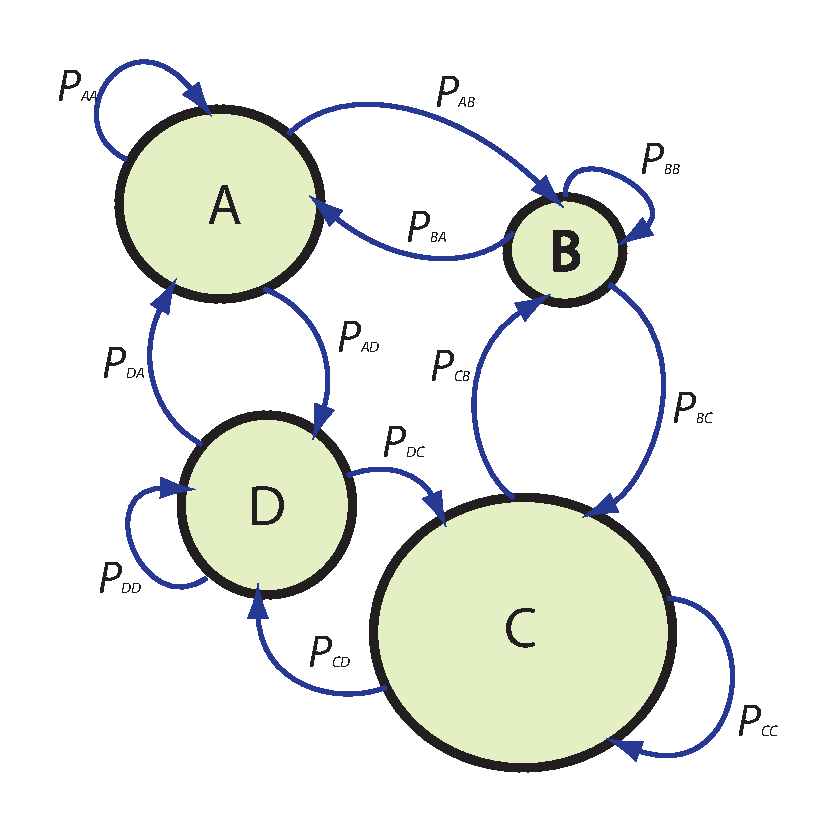
\includegraphics[scale=0.3]{generic-geographical-template.pdf}
			\end{column}
			\begin{column}[T]{0.01 \textwidth}
				{\LARGE  ${\Longrightarrow}$ }
			\end{column}
			\begin{column}[c]{0.40 \textwidth}	
			    \begin{tabular}{c|cccc}
			          & A & B & C & D\\
					\hline	             
			        A & $P_{AA}$ & $P_{AB}$ & $P_{AC}$ & $P_{AD}$ \\
			        B & $P_{BA}$ & $P_{BB}$ & $P_{BC}$ & $P_{BD}$ \\
			        C & $P_{CA}$ & $P_{CB}$ & $P_{CC}$ & $P_{CD}$ \\
			        D & $P_{DA}$ & $P_{DB}$ & $P_{DC}$ & $P_{DD}$ \\
		        \end{tabular}
			\end{column}	        
		\end{columns}
	\end{block}
\end{frame} 

\begin{frame}
	\frametitle{Speciation Modes}
	\begin{itemize}
		\item Sympatric \\
			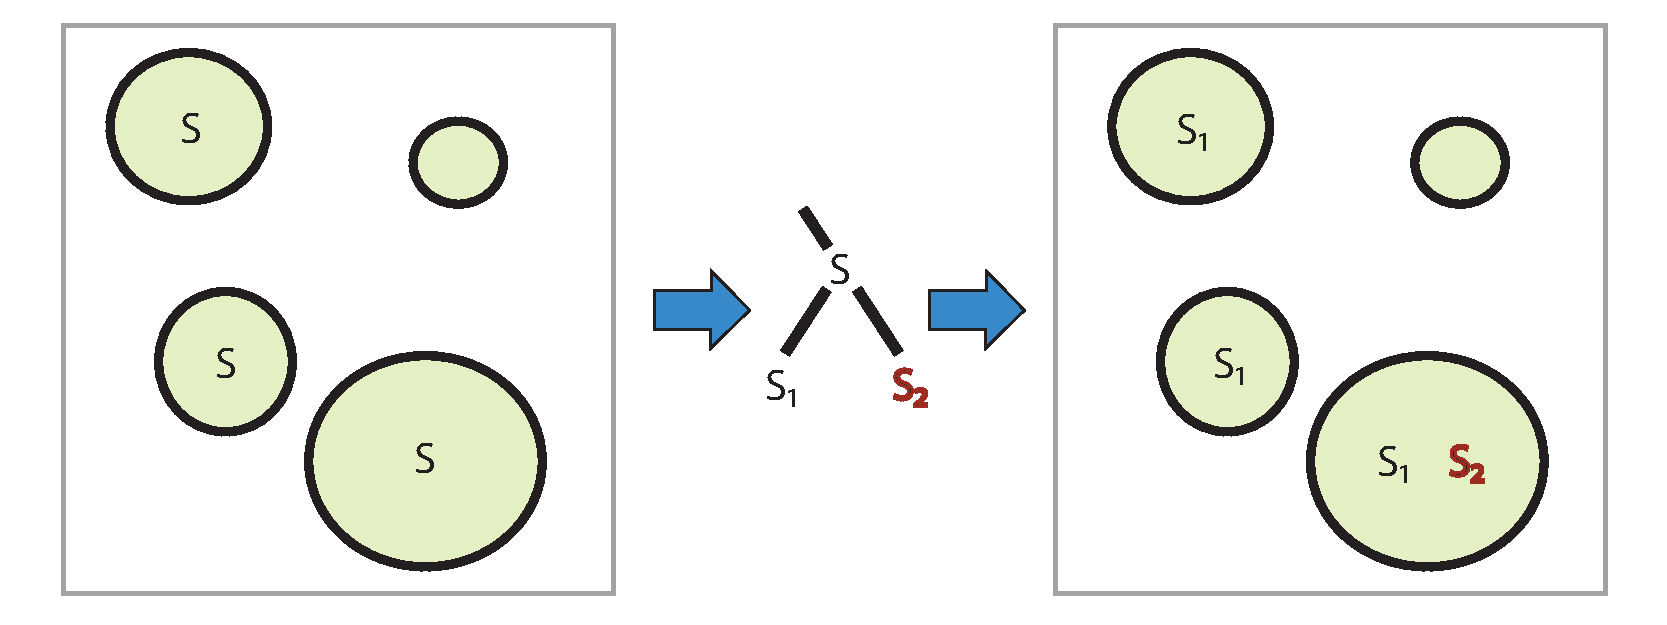
\includegraphics[scale=0.3]{sympatric-speciation.pdf}
		\item Allopatric \\
			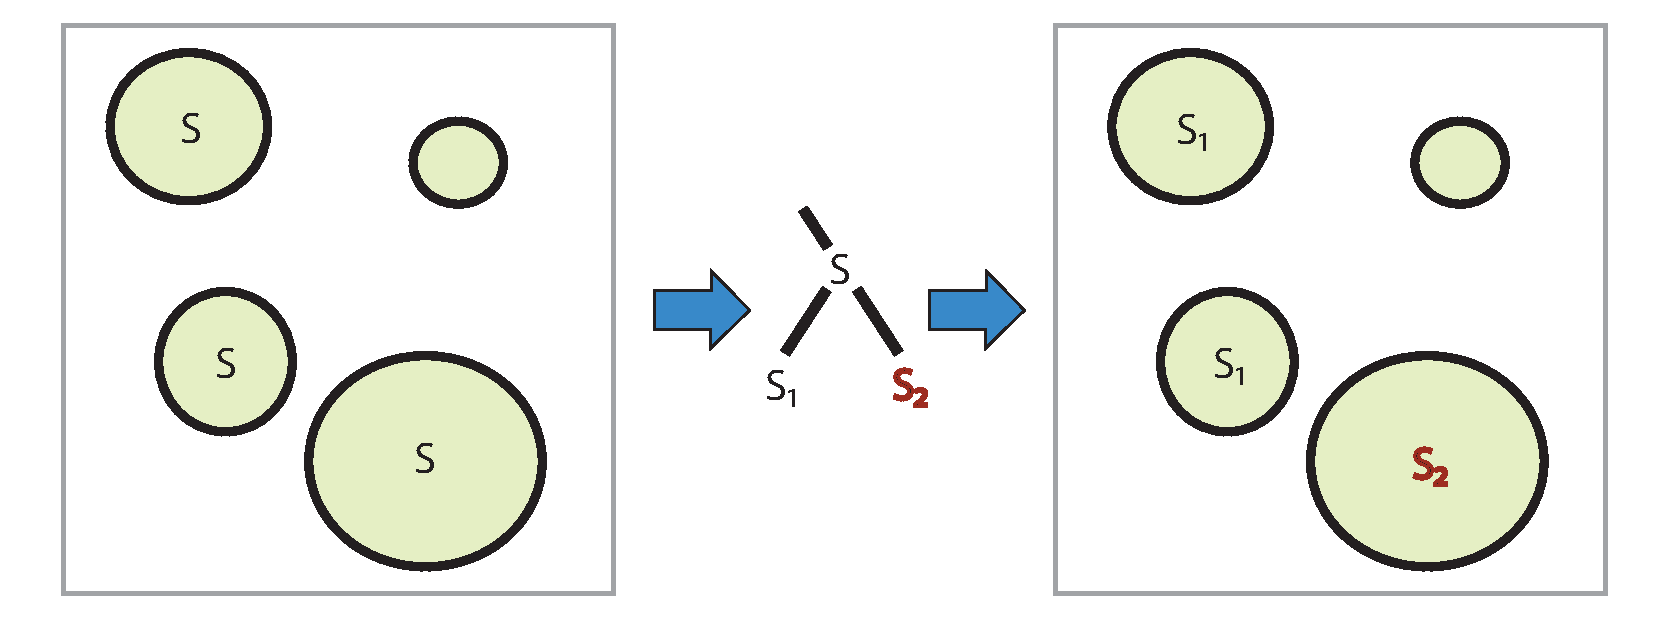
\includegraphics[scale=0.3]{allopatric-speciation.pdf}			
	\end{itemize}
\end{frame}

\begin{frame}
	\frametitle{Simulation Set Up}		
		\begin{itemize}
			\item Set model parameters:
				\begin{itemize}
					\item Birth (speciation) rate, $\lambda$.
					\item Death (extinction) rate, $\mu$.
					\item Geographic template.
					\item Speciation mode.
				\end{itemize}				
		   \item Set termination condition:
				\begin{itemize}
					\item Target diversity: run until total number of species = $T$.
					\item Number of generations: run until number of generations = $G$.
				\end{itemize}						
			\item Specify random number seed.							
		\end{itemize}									
\end{frame}


\begin{frame}
	\frametitle{Simulation Procedure}
	\begin{enumerate}
		\item Initialize: introduce single lineage into a region.
		\item Repeat until $T$ species or $G$ generations, or all species extinct:
			\begin{itemize}
				\item Migration:			
				\begin{itemize} 
					\item For each species in each region, select a destination region for dispersal (including current region, i.e., no dispersal) according to dispersal probability.
					\item Add species to destination region if not already present.
				\end{itemize}
			
				\item Diversification:
				\begin{itemize}	 
					\item For each species in the system, draw a uniform random number, $u \sim U(0,1)$.					
					\item If $u < \lambda$: split lineage.
					\item If $u > \lambda$ and $u < (\lambda + \mu)$: remove lineage.
				\end{itemize}	
			\end{itemize}
		\item Report results.					
	\end{enumerate}
\end{frame}

\begin{frame}
	\frametitle{Simulation Output}
	\begin{itemize}
		\item Incidence (presence/absence) matrix.
		\item Phylogeny.
		\item Summary of total number of lineages and total number of endemic lineages in each region.
		\item Classification tree of areas based on shared species.
	\end{itemize}
\end{frame}



\end{document}






